\documentclass[review]{elsarticle}

\usepackage{lineno,hyperref}
\modulolinenumbers[5]

\journal{Journal of \LaTeX\ Templates}

%%%%%%%%%%%%%%%%%%%%%%%
%% Elsevier bibliography styles
%%%%%%%%%%%%%%%%%%%%%%%
%% To change the style, put a % in front of the second line of the current style and
%% remove the % from the second line of the style you would like to use.
%%%%%%%%%%%%%%%%%%%%%%%

%% Numbered
%\bibliographystyle{model1-num-names}

%% Numbered without titles
%\bibliographystyle{model1a-num-names}

%% Harvard
%\bibliographystyle{model2-names.bst}\biboptions{authoryear}

%% Vancouver numbered
%\usepackage{numcompress}\bibliographystyle{model3-num-names}

%% Vancouver name/year
%\usepackage{numcompress}\bibliographystyle{model4-names}\biboptions{authoryear}

%% APA style
%\bibliographystyle{model5-names}\biboptions{authoryear}

%% AMA style
%\usepackage{numcompress}\bibliographystyle{model6-num-names}

%% `Elsevier LaTeX' style
\bibliographystyle{elsarticle-num}
%%%%%%%%%%%%%%%%%%%%%%%

\begin{document}

\begin{frontmatter}

\title{A mixed-dimensional model for the simulation of soil thermal hydrology in polygonal tundra: Proof-of-concept simulations}
\tnotetext[mytitlenote]{Fully documented templates are available in the elsarticle package on \href{http://www.ctan.org/tex-archive/macros/latex/contrib/elsarticle}{CTAN}.}

%% Group authors per affiliation:
%\author{Elsevier\fnref{myfootnote}}
%\address{Radarweg 29, Amsterdam}
%\fntext[myfootnote]{Since 1880.}

%% or include affiliations in footnotes:
%\author[mymainaddress,mysecondaryaddress]{Elsevier Inc}
%\ead[url]{www.elsevier.com}

%\author[mysecondaryaddress]{Global Customer Service\corref{mycorrespondingauthor}}
%\cortext[mycorrespondingauthor]{Corresponding author}
%\ead{support@elsevier.com}

%\address[mymainaddress]{1600 John F Kennedy Boulevard, Philadelphia}
%\address[mysecondaryaddress]{360 Park Avenue South, New York}

\begin{abstract}


Approximately one-quarter of the land surface in the Northern Hemisphere is occupied by permafrost -- permanently frozen ground.  Permafrost harbors massive amount of frozen organic carbon and is warming at a rate significantly larger than the rest of the planet. These permafrost regions may become another source of carbon emission to the atmosphere upon thawing.
Simulating soil thermal hydrology in degrading permafrost regions is challenging because of strong coupling among thermal and hydrologic processes on the surface and in the subsurface. The purpose of this work is to present a novel mixed-dimensional model to make these process-rich simulations tractable at watershed scales. The approach indirectly couples one-dimensional subsurface columns with a two-dimensional surface system. The strategy of discretizing subsurface as independent columns and then coupling indirectly through surface flow system is strongly motivated by fine-scale simulations. The fine-scale simulations explored considerable variations in thermal conditions among the centers, rims, and troughs of ice-wedge polygons during the summer; mainly equilibrated by lateral heat transport. We have implemented this novel structure in the state-of-art Arctic Terrestrial Simulator (ATS) to simulate the thermal hydrology of thawing polygonal tundra near Barrow, Alaska in warming climate.
Our loosely coupled scheme for this mixed-dimensional modeling strategy involves two steps. First we solve overland thermal hydrology system (two-dimensional surface system) with no sources ? act as a spatial distributor of the surface pressure and temperature. The solution of the surface system serves as initial condition for the subsurface system. That is, the surface system updates the subsurface system (one-dimensional columns) before the subsurface system advances in time. Then, we implicitly solve subsurface system with surface ponding but no surface lateral flow, and use the output of that half-step to update surface pressure and temperature for the next time step in the algorithm. The numerical results of our loosely coupled scheme are comparable to the fully implicit (strongly coupled) scheme. We demonstrate the accuracy, efficiency, and time convergence analysis of our scheme.
Most of the available multiphysics simulators don?t support this kind of mixed-dimensional modeling techniques, and are capable to work with a single spatial domain -- that limits the usage of those simulators at larger scales with the complexities of the physical, chemical, biological and geological processes and strong coupling among them. This is a very first attempt to couple state-of-the-art representation of freezing soil physics with overland flow and surface energy balance at scales of 10s of meters. The scheme is computationally less expensive, respects the accuracy and scalability, and applicable to many integrated surface/subsurface thermal hydrology at field-scale. The other exciting features of the strategy include efficient tracking of thaw-induced subsidence and easy sub-cycling of physical processes. Moreover, it avoids any mesh tangling and poor mesh quality that can result from representing dynamic topography in a three-dimensional simulation.
\end{abstract}
\begin{keyword}
Mixed-dimensional model\sep Permafrost dynamics  \sep Process-rich simulations \sep Arctic   \sep Field-scale projections  
%\MSC[2010] 00-01\sep  99-00
\end{keyword}

\end{frontmatter}

\linenumbers

\section{Introduction}
A massive amount of organic carbon is stored in perennially frozen soil called permafrost. The Northern Hemisphere hosts approximately 1672 Pg of organic carbon and these high-latitude regions are warming at a rate considerably faster than in the most of the world (Tarnocai et al., 2009; Hansen et al. 1999; Turner et al., 2007; Arctic Climate Impact Assessment, 2004). In warming climate, permafrost regions are under potential risk of carbon release to the atmosphere. With increase in the temperature these permafrost regions will turn from a carbon sink to a carbon source that will increase the concentration of carbon in the atmosphere, which in turn leads to further increase in the temperature. Permafrost covers about 25\% of the land surface in the Northern Hemisphere (Brown et al. 1997) and upon thawing would cause significant changes in the surface/subsurface thermal hydrology (Walvoord and Striegl 2007; Lyon et al. 2009; IPCC 2014).

There has been a great interest in studying permafrost dynamics in warming climate through modeling and simulation techniques. If on one side, these tools help to gain insight into the role of soil warming, its consequences on the degradation of permafrost and the associated changes in the surface/subsurface thermal hydrology, but on the other hand simulating permafrost dynamics with all the surface/subsurface processes and interactions (coupling) among them at larger scales is a hard and an important challenge. The work in 70-80's mostly focused on better understanding of infiltration processes (Nakano and Brown, 1971; Harlen 1973; Guymon and Luthin, 1974; Jame and Norum, 1980). In the previous decade we find some simplified coarse-scale surface modeling attempts (Takata et al. 2003; Ling and Zhang, 2004; Nicolsky et al., 2007; McKenzie et al., 2007), and recently a few three-dimensional simulations with simplified models have demonstrated permafrost dynamics (Bense et al. 2009; Painter, 2011; Lawrence et al. 2011; Koven et al. 2013). Simplified hydrological simulations may not capture the profound impact of permafrost thawing on surface/subsurface hydrology. (Incomplete ??)

Therefore, it is desirable to have more detailed and sophisticated hydrological computer codes to simulate fully integrated surface/subsurface system over long temporal and spatial domains. However, as said earlier, simulating soil thermal hydrology in degrading permafrost regions is challenging due to strong coupling among thermal and hydrologic process on the surface and in the subsurface. Frozen subsurface blocks infiltration, as ice begins to melt (phase change), the soil hydraulic conductivity increases, consequently, the time-step of the numerical methods decreases.  For long term projections of permafrost dynamics, a small time-step is not practical. A huge amount of computational time is spent in recovering the time-step, which may not recover in a reasonable amount of time. A sophisticated simulator, in addition to handling the complexities of the hydrological and thermal processes and coupling among them, should also be capable of  tracking subsurface subsidence when simulating permafrost dynamics. Most of the hydrological simulators are designed for conducting three-dimensional simulations, however, deformations in a three-dimensional simulation are not easy to track due to mesh tangling and could cost huge computational burden.

To address the above mentioned computational challenges, we present a multipurpose novel mixed-dimensional modeling technique for the process-rich simulations of integrated surface/subsurface permafrost thermal hydrology. The new modeling strategy has also some additional unique capabilities, for example, easy and efficient subcycling of a particular region of the computational domain. The approach indirectly couples individual (one-dimensional) ice-wedge polygons that discretize the horizontal landscape to two-dimensional surface system. The implementation of a mixed-dimensional model requires a coupling scheme that provides interaction at the interface between different dimensions. In this work, we loosely couple the two-dimensional surface system with subsurface polyhedra that are treated as one-dimensional columns. The loosely coupled scheme has two main step. First, overland thermal hydrology system (two-dimensional surface system) is solved without external and exchanged sources. The second step solves subsurface system with surface ponding but no lateral surface flow. The first step acts as a spatial distributor of the surface pressure and temperature, and its solution serves as initial condition for the second step. That is, the surface system updates the subsurface system (one-dimensional columns) before the subsurface system advances in time. After the update from the first step, we implicitly solve subsurface system with surface ponding but no surface lateral flow, and use the output of that half-step to update surface pressure and temperature for the next time step in the algorithm. 

This mixed-dimensional modeling approach is motivated by some fine-scale simulations of the permafrost regions. Fine-scale simulations showed significant differences in the thermal conditions among centers, rims and troughs of ice-wedge polygons, largely equilibrated by the lateral heat transport during summer, thereby an intermediate-scale representation is more practical and appropriate at the larger scales; more details are presented later in the paper. Though this modeling capability has broader scope but here we mainly focus on simulating permafrost thermal hydrology in polygonal tundra near Barrow, Alaska. 

We have implemented our mixed-dimensional modeling strategy in the open-source state-of-the-art software Arctic Terrestrial Simulator (ATS) (Coon et. al, 2016; Painter et. al., 2015).  Particularly related to this work, ATS solves strongly coupled surface energy balance and surface/subsurface thermal hydrology in a highly parallel 3D environment. ATS leverages Amanzi (Moulton et. al., 2012) capabilities. The Amanzi is a flow and reactive transport simulator mainly build on the Arcos framework. Arcos is a multiphysics management framework based on a Multiprocess Coordinator (MPC) architecture. The MPCs in the Arcos framework couple many single processes to construct a complex hierarchical structure thus allows state-of-the-art modeling technique. The flexibility and extensibility features of the Arcos framework efficiently enables a computationally advantageous modeling strategy that we present here which otherwise could not have been possible with traditional simulators.

The paper is organized as follows: Section 2 presents the mixed-dimensional modeling approach, and some fine-scale simulations? results and analysis that motivated the approach. Section 3 highlights the Arctic Terrestrial Simulator (ATS) and the Arcos framework for the implementation of the model. Section 4 describes time-convergence analysis, scalability of the technique and comparison of the numerical results with the implicit scheme. Concluding remarks and future research are offered in Section 5, followed by references.

\section{Motivation and Modeling Approach}

\subsection{Motivation: Fine-scale Simulation Study}
TODO

\section{Arcos Framework and Refactoring Strategy}
As stated earlier, studying permafrost dynamics at large-scale is an important challenge, and requires simulators to be capable of handling many surface and subsurface processes, and the mutual interactions among them. Most existing hydrological computer codes, in the context of implicit-based coupling among processes, and the implementation architecture, don?t efficiently allow and encourage modelers to study permafrost evolution at larger spatial and temporal scales. These simulators lack the flexibility of future development for extensions, that is, bringing more processes and/or increasing the complexity of models for more accurate representation of reality) is not a trivial task.

To address the above mentioned and other challenges we face in the existing simulators, we use Arcos framework. The Arcos framework manages the process kernels (a mathematical model) in a hierarchical way (i.e., process tree form). In other words, the Arcos framework provides an architecture that manages multiphysics models and allow them to interact through a Multiprocess Coordinator (MPC). This hierarchical structure keeps the implementation of each mathematical model isolated that can be used (for coupling purpose) with many other models through an MPC. Due to this flexibility and significant extensibility, the Arcos framework-based simulators provide ideal modeling environment, tackle the complexities efficiently, and encourage future extensions. 
We use an open-source state-of-the-art computer code the Arctic Terrestrial Simulator (ATS). The ATS is inherited from Amanzi (a simulator for flow and reactive transport.) The Amanzi and hence the ATS architecture is based on the Arcos framework.  Below we describe how we refactored the ATS for our modeling technique. [Add a picture of simple process tree??]


\subsection{Coupling and Mixed-Dimensional Modeling Approach}
The loosely coupled scheme for analyzing our mixed-dimensional model involves two fundamental steps. As depicted in Fig.~\ref{coupling-schematic}, step 1 solves overland thermal hydrology system with no sources, hereafter referred to as surface-star system. It role is to spatially distribute the surface pressure and temperature over 2D surface domain, and updates subsurface at the interface, that is, initializes the subsurface system. In other words, the surface-star system updates the subsurface system before the subsurface system advances in time. In the second step, a fully implicitly subsurface system with surface ponding but no surface lateral flow is solved. Finally, the output of this half-step updates surface pressure and temperature for the next time step in the algorithm. To avoid confusion from now on, we will refer to the pressures and temperatures of step 2 as the subsurface and surface pressures and temperatures, while that of step 1 will be called as surface-star pressure and surface-star temperature.

\begin{figure}[!htpb]
\centering
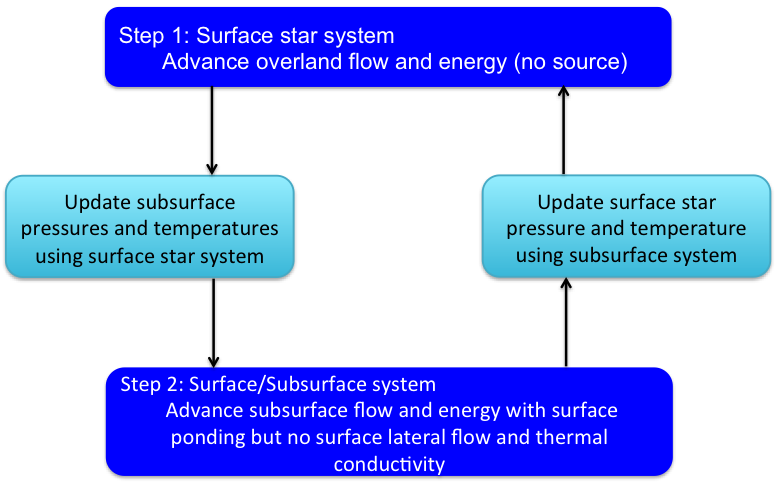
\includegraphics[height = 6.5cm, width=11cm]{figures/shematic-couplingscheme1.png}
\caption{Schematic of the loosely coupled scheme for our mixed-dimensional model.}
\label{coupling-schematic}
\end{figure}



In our modeling strategy, we treat each subsurface column independently and the interaction among the 1D subsurface columns, the surface system (technically a surface cell on top of 1D subsurface columns for water ponding) and the 2D surface star system happens through a coupling algorithm. Technically, the strategy splits the 3D domain into N subdomains for subsurface columns, N for surface system, and one subdomain for the surface-star system. In total, 2N+1 subdomains are required that form a complex process-kernel (PK) tree with 2N+1 processes. Fig.~\ref{pk-tree} shows a process tree that consists of independent models, strongly  and weakly coupled PKs highlighted in different colors.  

\begin{figure}[!htpb]
\centering
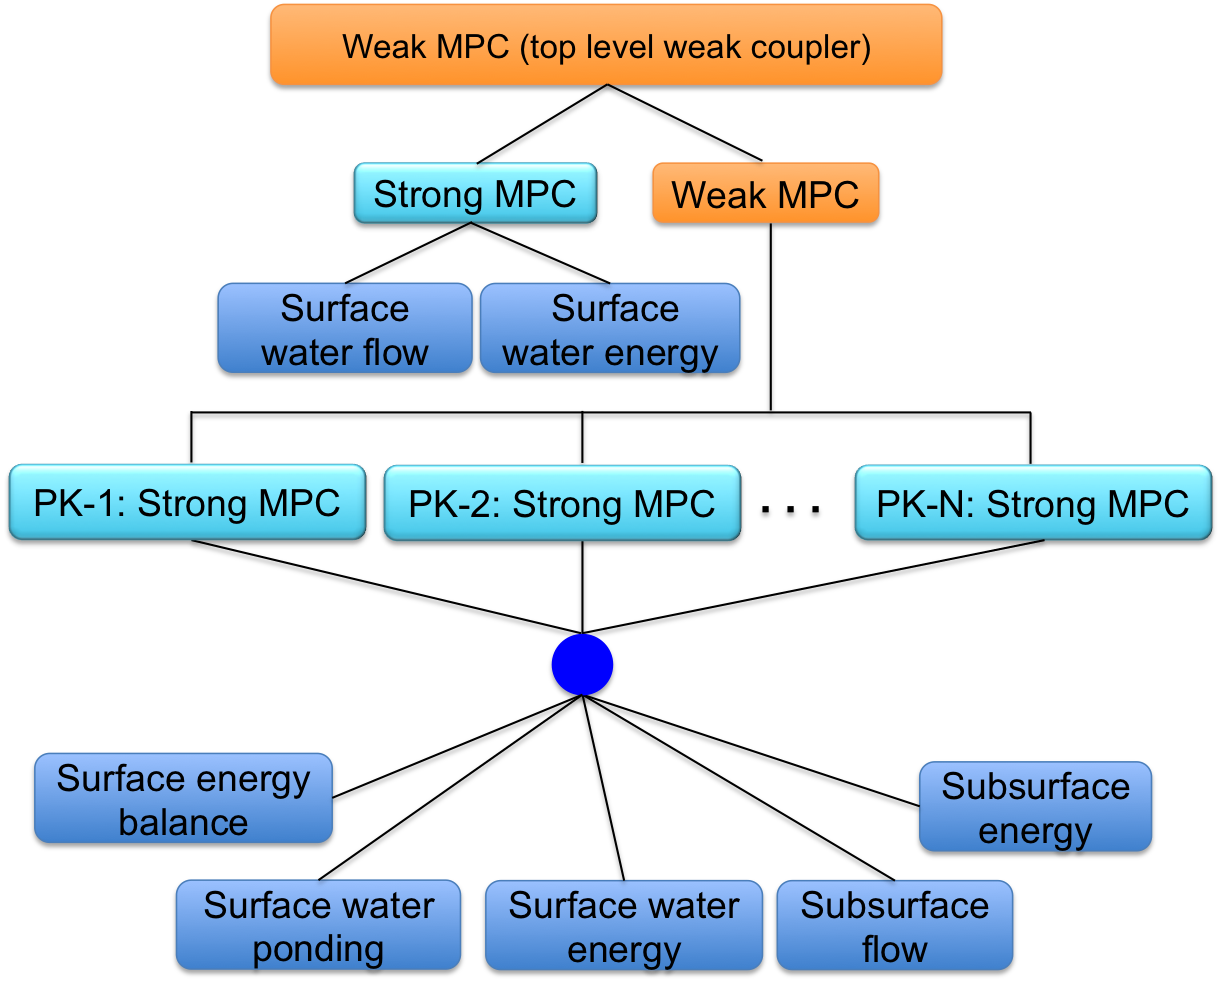
\includegraphics[height = 9.5cm, width=11cm]{figures/process-tree.png}
\caption{A customized hierarchical structure of the process kernels. Blue blocks highlights independent process models; Light blue blocks strongly couple indepdent process kernels; Orange blocks represent weak couplers.}
\label{pk-tree}
\end{figure}

The pressure and temperature updates in the weakly coupled scheme (see, Fig.~\ref{coupling-schematic}) occur at the top level weak MPC as presented in Fig.~\ref{pk-tree}. At level 2, the strong MPC advances the surface-star system in time and afterwards passses the control to the weak MPC (to the left). The weak MPC at level 2 sequentially executes surface and subsurface processes. Each PK (strong MPC) at level 3 is an integrated system of the surface and subsurface subdomains, 2N subdomains in total. Finally, each strong MPC (at level 3) advances the PKs at the lowest level on their corresponding subdomains. 

The ATS was significantly refactored to accommodate the above customized weak MPC. The refactoring allows PKs to be replicated across multiple subdomains (meshes), that is, each PK is state independent. This stateless structure permits each surface and subsurface subdomain to have its own domain name, say 
column$\_n$, surface$\_$column$\_n$, $n=1,2,3, \dots$,N. In fact, the refactoring strategy prefixes the variables (both independent and dependent) with their corresponding subdomain names, e.g., column$\_n$-pressure, column$\_n$-temperature, $n=1,2,3, \dots$, N.

The complexity of the multiphysics PK tree in our modeling strategy could not have been achieved without the Arcos framework. Though the complexity in the PK tree is evident but additional complications are intended as we include more processes (physical, chemical, biological and geological processes) and their mutual interactions. All these processes are equally important for an accurate and reliable long-term projections of permafrost degradation. That said, the refactored ATS provides an effective and sophisticated tool that can be used to address the important challenges in the permafrost thawing in the warming climate.


\section{Numerical Tests and Discussions}

In this section, we begin with the discussion of a few numerical experiments that have been carried out to test the code development and verify the physical behavior of the refactored modules (PKs) of the ATS. We test each individual PK standalone and the compare its results with 3D simulation results, prior to coupling with other refactored PKs. Finally, all refactored PKs are coupled to construct a process tree (hierarchy of PKs) yielding the coupling scheme for our mixed-dimensional model.
We describe the spinup process (i.e., model's initialization), and present a speedup study along with highlighting its computational efficiency in comparison with other scheme. Finally, we switch to demonstrate the time convergence analysis of our scheme. Numerical results of 3D simulations are used as a reference. This section reveals our approximation of 3D models is accurate, robust, and more practical for studying permafrost dynamics. The accuracy, efficiency, and incorporation of all the important physical processes make it highly applicable for long-term projections of Arctic regions.

We have performed a series of tests at the development stage to ensure the accuracy and time-convergence of our model, and compared our results against numerical solution of three-dimensional model. In 3D models the surface and subsurface systems are strongly coupled and solved implicitly. Since our model required major refactoring of the ATS, so individual pieces of the code were deeply tested before integration -- they are listed below:
\begin{itemize}
\item{ Problem Test 1 (Subsurface Flow): \\
We consider multiple subsurface columns with flat top surface -- each column is an independent domain. Put water table below the surface, infiltrates and fills the subsurface columns.
}
\item{ Problem Test 2 (Surface and Subsurface Flow only): \\
This is an extension of the Test 1. We Put water table below the surface. Water infiltrates and fill subsurface columns prior to surface ponding. 
}

\item{ Problem Test 3 (Subsurface Thermal Hydrology): \\
Here we add energy equation to Test 1. Initially we establish water table close to the surface, and start freezing from below. The frozen subsurface columns are thawed from the top.}

\item{ Problem Test 4 (Surface and Subsurface Thermal Hydrology) \\
In this test, we incorporate surface thermal hydrology into Test 3. A warm rain precipitation thaws the subsurface columns, saturate them and afterwards ponds on the surface.}

\item{ Problem Test 5 (Surface Energy Balance, Surface and Subsurface Thermal Hydrology) \\
A fully integrated surface/subsurface processes test. We introduce an energy balance equation to Test 4. An initially established ice table below the surface has been thawed by warm rain, incoming-short radiation and air temperature.}

\end{itemize}
Due to symmetry in the domains of above numerical tests, that is, the subsurface columns are copies of each other and surface is flat, we get identical results and compare very well with its corresponding three-dimensional simulation results. Passing all the above tests conclude refactoring of the ATS a success. In the preceding discussion, we consider general polyhedra to demonstrate the efficiency and accuracy of our scheme.


\subsection{Spinup Process}
Spinup refers to a sequential process that initializes model's domain to make it consistent with current climate before driving it with meteorological forcing data for future projections. We take the following steps to spinup the model:
\begin{itemize}
\item{ Step 1. Establish a water table close to the surface in a one-dimensional subsurface column by running a steady-state Richards flow.}
\item{Step 2. Freeze the water table from below (set the bottom boundary condition below freezing) leading to an ice table in the subsurface. The level of the ice table depends on the location of the water table established in step 1. With a phase change (water to ice), the ice table is relatively higher than the water table in the subsurface column. Therefore, from the numerical point of view, the idea is to place the water table at a location such that the ice table remains below the surface.}
\item{Step 3. Initialize the entire subsurface domain using one-dimensional column data, that is, establish an ice table in the entire domain using single column data obtained in step 2. 
%ATS has an option for initializing the whole subsurface domain using 1D subsurface column data. That is why, in the above two steps we consider a 1D column.
}
\item{Step 4. Drive the model for 10 years -- a cyclic simulation with one year averaged meteorological data. The one year averaged data is obtained by aggregating the 10 years observed meteorological data, that is, the mean value of a forcing factor (say, air temperature, humidity etc.) for a specific day per 10 years. This completes a typical spinup process in ATS, that is, initialization of the model is done. Lastly, the reason for driving the model simulation for 10 years is based on the available observed data from 1998 to 2009 at Barrow, Alaska -- the site of our interest in this work.}
 \end{itemize}
 \subsection {Time Convergence Studies : 75 polygons}           
 
Pertaining to accuracy,  it is desirable to compare numerical results of the mixed-dimensional model against fully coupled three-dimensional simulations. We consider a region 40 m deep, 173 m long and 43 m wide in the Barrow, Alaska, see Fig.~\ref{surf-location}. The domain is a part of the low-gradient polygonal tundra that consist of 75 general polyhedra. We initialize the model using the spinup process described above. As highlighted in Fig.~\ref{surf-location}, we select five spots to perform a location-based comparison of the numerical results of the two schemes. After initialization we project the permafrost evolution to 2100.

Meteorological data discussion: air temperature; humidity etc put some images

 \begin{figure}[!htpb]
\centering
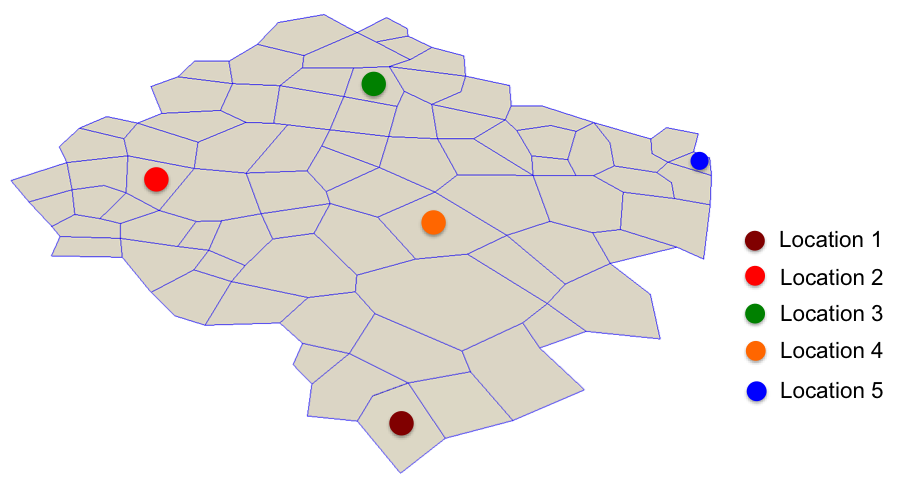
\includegraphics[height = 5.5cm, width=9cm]{figures/surface-locations.png}
\caption{An illustration of the five spatial locations on 75 polygons cluster for location-based comparison of the two schemes. Location 1: Outlet. Location 2: High elevated spot. Location 3-4: Intermediate elevation spots. Location 5: Lowest elevation spot.}
\label{surf-location}
\end{figure}

\subsection{Speedup Study}
The new modeling approach significantly reduces the computational time. We discuss two aspects of the efficiency that we achieve with our modeling technique: (i) How the simulation time improves in comparison with three-dimensional simulations; (ii) how efficiently it scales? Figs. X compare the computational time of the two modeling approaches for the domain consisting 75 polyhedra as shown in Fig Y. It has been experienced that 3D simulations require 16 times more computational resources than our approach. That is, the time taken by a serial run with our approach requires 16 processors to get a 3D simulation done in the same amount of time. Further, for a fixed number of processors, the computational time decrease by a factor of about 4 with our modeling technique. This is a huge computational advantage without sacrificing the numerical accuracy. We expect a considerable improvement pertaining to computational time and resources when we move to much larger domains. To recall, simulating process-rich permafrost dynamics at watershed-scale is a core reason behind this work. We show a speedup study of our modeling approach in Fig X. It shows assigning 3-5 subsurface columns to each processor gives the maximum speedup. Ideally, one would want to have a single subsurface column per processor to achieve the maximum efficiency, however, with increasing the number of processors, the cost of communication in the overhead 2D domain (i.e., the surface star system) limit the number of columns per processor. The surface star system is a simple 2D domain and definitely don?t require too many processors. 

Projection to 2100


\section{Conclusions}
 
\section{Future Directions}
Subcycling \\
Subgrid model, dynamic microtopography \\
Biogeochemistry \\
Thaw-induced subsidence \\
Whatelse?? 


\section{Bibliography styles}

%Here are two sample references: \cite{Feynman1963118,Dirac1953888}.

\section*{References}

\bibliography{mybibfile}

\end{document}